

% *** Authors should verify (and, if needed, correct) their LaTeX system  ***
% *** with the testflow diagnostic prior to trusting their LaTeX platform ***
% *** with production work. IEEE's font choices can trigger bugs that do  ***
% *** not appear when using other class files.                            ***
% The testflow support page is at:
% http://www.michaelshell.org/tex/testflow/


%%%%%%%%%%%%%%%%%%%%%%%%%%%%%%%%%%%%%%%%%%%%%%%%%%%%%%%%%%%%%%%%%%%
%%%%%%%%%%%%%%%%%%%%%%%%%%%%%%%%%%%%%%%%%%%%%%%%%%%%%%%%%%%%%%%%%%%
\documentclass[conference,compsoc]{IEEEtran}
% Add the compsoc option for Computer Society conferences.
%%%%%%%%%%%%%%%%%%%%%%%%%%%%%%%%%%%%%%%%%%%%%%%%%%%%%%%%%%%%%%%%%%%
%%%%%%%%%%%%%%%%%%%%%%%%%%%%%%%%%%%%%%%%%%%%%%%%%%%%%%%%%%%%%%%%%%%


% *** CITATION PACKAGES ***
%
\usepackage{cite}

% *** GRAPHICS RELATED PACKAGES ***
%
\ifCLASSINFOpdf
  \usepackage[pdftex]{graphicx}
  % declare the path(s) where your graphic files are
  % \graphicspath{{../pdf/}{../jpeg/}}
  % and their extensions so you won't have to specify these with
  % every instance of \includegraphics
  % \DeclareGraphicsExtensions{.pdf,.jpeg,.png}
\else
  % or other class option (dvipsone, dvipdf, if not using dvips). graphicx
  % will default to the driver specified in the system graphics.cfg if no
  % driver is specified.
  \usepackage[dvips]{graphicx}
  % declare the path(s) where your graphic files are
  % \graphicspath{{../eps/}}
  % and their extensions so you won't have to specify these with
  % every instance of \includegraphics
  % \DeclareGraphicsExtensions{.eps}
\fi
% graphicx was written by David Carlisle and Sebastian Rahtz. It is
% required if you want graphics, photos, etc. graphicx.sty is already
% installed on most LaTeX systems. The latest version and documentation can
% be obtained at:
% http://www.ctan.org/tex-archive/macros/latex/required/graphics/
% Another good source of documentation is "Using Imported Graphics in
% LaTeX2e" by Keith Reckdahl which can be found as epslatex.ps or
% epslatex.pdf at: http://www.ctan.org/tex-archive/info/
%
% latex, and pdflatex in dvi mode, support graphics in encapsulated
% postscript (.eps) format. pdflatex in pdf mode supports graphics
% in .pdf, .jpeg, .png and .mps (metapost) formats. Users should ensure
% that all non-photo figures use a vector format (.eps, .pdf, .mps) and
% not a bitmapped formats (.jpeg, .png). IEEE frowns on bitmapped formats
% which can result in "jaggedy"/blurry rendering of lines and letters as
% well as large increases in file sizes.
%
% You can find documentation about the pdfTeX application at:
% http://www.tug.org/applications/pdftex


% *** MATH PACKAGES ***
%
\usepackage[cmex10]{amsmath}
% Also, note that the amsmath package sets \interdisplaylinepenalty to 10000
% thus preventing page breaks from occurring within multiline equations. Use:
%\interdisplaylinepenalty=2500
% after loading amsmath to restore such page breaks as IEEEtran.cls normally
% does. amsmath.sty is already installed on most LaTeX systems. The latest
% version and documentation can be obtained at:
% http://www.ctan.org/tex-archive/macros/latex/required/amslatex/math/
\usepackage{amsthm}
\usepackage{amsfonts}
\usepackage{amssymb}
\usepackage{latexsym}
\usepackage{epstopdf}


% *** SPECIALIZED LIST PACKAGES ***
%
\usepackage{algorithmic}
% algorithmic.sty was written by Peter Williams and Rogerio Brito.
% This package provides an algorithmic environment fo describing algorithms.
% You can use the algorithmic environment in-text or within a figure
% environment to provide for a floating algorithm. Do NOT use the algorithm
% floating environment provided by algorithm.sty (by the same authors) or
% algorithm2e.sty (by Christophe Fiorio) as IEEE does not use dedicated
% algorithm float types and packages that provide these will not provide
% correct IEEE style captions. The latest version and documentation of
% algorithmic.sty can be obtained at:
% http://www.ctan.org/tex-archive/macros/latex/contrib/algorithms/
% There is also a support site at:
% http://algorithms.berlios.de/index.html
% Also of interest may be the (relatively newer and more customizable)
% algorithmicx.sty package by Szasz Janos:
% http://www.ctan.org/tex-archive/macros/latex/contrib/algorithmicx/





%\usepackage{mdwmath}
%\usepackage{mdwtab}
% Also highly recommended is Mark Wooding's extremely powerful MDW tools,
% especially mdwmath.sty and mdwtab.sty which are used to format equations
% and tables, respectively. The MDWtools set is already installed on most
% LaTeX systems. The lastest version and documentation is available at:
% http://www.ctan.org/tex-archive/macros/latex/contrib/mdwtools/


% IEEEtran contains the IEEEeqnarray family of commands that can be used to
% generate multiline equations as well as matrices, tables, etc., of high
% quality.





% *** SUBFIGURE PACKAGES ***
%\usepackage[tight,footnotesize]{subfigure}
% subfigure.sty was written by Steven Douglas Cochran. This package makes it
% easy to put subfigures in your figures. e.g., "Figure 1a and 1b". For IEEE
% work, it is a good idea to load it with the tight package option to reduce
% the amount of white space around the subfigures. subfigure.sty is already
% installed on most LaTeX systems. The latest version and documentation can
% be obtained at:
% http://www.ctan.org/tex-archive/obsolete/macros/latex/contrib/subfigure/
% subfigure.sty has been superceeded by subfig.sty.



%\usepackage[caption=false]{caption}
%\usepackage[font=footnotesize]{subfig}
% subfig.sty, also written by Steven Douglas Cochran, is the modern
% replacement for subfigure.sty. However, subfig.sty requires and
% automatically loads Axel Sommerfeldt's caption.sty which will override
% IEEEtran.cls handling of captions and this will result in nonIEEE style
% figure/table captions. To prevent this problem, be sure and preload
% caption.sty with its "caption=false" package option. This is will preserve
% IEEEtran.cls handing of captions. Version 1.3 (2005/06/28) and later
% (recommended due to many improvements over 1.2) of subfig.sty supports
% the caption=false option directly:
%\usepackage[caption=false,font=footnotesize]{subfig}
%
% The latest version and documentation can be obtained at:
% http://www.ctan.org/tex-archive/macros/latex/contrib/subfig/
% The latest version and documentation of caption.sty can be obtained at:
% http://www.ctan.org/tex-archive/macros/latex/contrib/caption/




% *** FLOAT PACKAGES ***
%
%\usepackage{fixltx2e}
% fixltx2e, the successor to the earlier fix2col.sty, was written by
% Frank Mittelbach and David Carlisle. This package corrects a few problems
% in the LaTeX2e kernel, the most notable of which is that in current
% LaTeX2e releases, the ordering of single and double column floats is not
% guaranteed to be preserved. Thus, an unpatched LaTeX2e can allow a
% single column figure to be placed prior to an earlier double column
% figure. The latest version and documentation can be found at:
% http://www.ctan.org/tex-archive/macros/latex/base/



%\usepackage{stfloats}
% stfloats.sty was written by Sigitas Tolusis. This package gives LaTeX2e
% the ability to do double column floats at the bottom of the page as well
% as the top. (e.g., "\begin{figure*}[!b]" is not normally possible in
% LaTeX2e). It also provides a command:
%\fnbelowfloat
% to enable the placement of footnotes below bottom floats (the standard
% LaTeX2e kernel puts them above bottom floats). This is an invasive package
% which rewrites many portions of the LaTeX2e float routines. It may not work
% with other packages that modify the LaTeX2e float routines. The latest
% version and documentation can be obtained at:
% http://www.ctan.org/tex-archive/macros/latex/contrib/sttools/
% Documentation is contained in the stfloats.sty comments as well as in the
% presfull.pdf file. Do not use the stfloats baselinefloat ability as IEEE
% does not allow \baselineskip to stretch. Authors submitting work to the
% IEEE should note that IEEE rarely uses double column equations and
% that authors should try to avoid such use. Do not be tempted to use the
% cuted.sty or midfloat.sty packages (also by Sigitas Tolusis) as IEEE does
% not format its papers in such ways.





% *** PDF, URL AND HYPERLINK PACKAGES ***
%
%\usepackage{url}
% url.sty was written by Donald Arseneau. It provides better support for
% handling and breaking URLs. url.sty is already installed on most LaTeX
% systems. The latest version can be obtained at:
% http://www.ctan.org/tex-archive/macros/latex/contrib/misc/
% Read the url.sty source comments for usage information. Basically,
% \url{my_url_here}.





% *** Do not adjust lengths that control margins, column widths, etc. ***
% *** Do not use packages that alter fonts (such as pslatex).         ***
% There should be no need to do such things with IEEEtran.cls V1.6 and later.
% (Unless specifically asked to do so by the journal or conference you plan
% to submit to, of course. )




%%%%%%%%%%%%%%%%%%%%%%%%%%%%%%%%%%%%%%%%%%%%%%%%%%%%%%%%%%%
% My MACROS
%%%%%%%%%%%%%%%%%%%%%%%%%%%%%%%%%%%%%%%%%%%%%%%%%%%%%%%%%%%
%% MATH GENERIC NOTATIONS
\newcommand{\disp}{\displaystyle}
\newcommand{\ba}{\begin{array}}
\newcommand{\ea}{\end{array}}
\newcommand{\btab}{\begin{table}}
\newcommand{\etab}{\end{table}}
\newcommand{\bcen}{\begin{center}}
\newcommand{\ecen}{\end{center}}
\newcommand{\btabb}{\begin{tabular}}
\newcommand{\etabb}{\end{tabular}}
\newcommand{\bea}{\begin{eqnarray}}
\newcommand{\eea}{\end{eqnarray}}
\newcommand{\beqn}{\begin{equation}}
\newcommand{\eeqn}{\end{equation}}
\newcommand{\beqnt}{\begin{equation*}}
\newcommand{\eeqnt}{\end{equation*}}
\newcommand{\bex}{\begin{example}}
\newcommand{\eex}{\end{example}}
\newcommand{\dintl}{\disp\int\limits}
\newcommand{\dsuml}{\disp\sum\limits}
\newcommand{\suml}{\sum\limits}
\newcommand{\intl}{\int\limits}
\newcommand{\onlygap}{\,\,\,\,}
\newcommand{\imp}{\Rightarrow\,\,}

%%%%%%%%%%%%%%%%%%%%%%%%%%%%%%%%%%%%%%%%%%%%%%%%%%%%%%%%%%%%%%%%%
%%%%%%%%%%%%%%%%%%%%%%%%%%%%%%%%%%%%%%%%%%%%%%%%%%%%%%%%%%%%%%%%%
%%%%%%%%%%%%%%%%%%%%%%%%%%%%%%%%%%%%%%%%%%%%%%%%%%%%%%%%%%%%%%%%%
% PHD specific MACROS
%%%%%%%%%%%%%%%%%%%%%%%%%%%%%%%%%%%%%%%%%%%%%%%%%%%%%%%%%%%%%%%%%
%%%%%%%%%%%%%%%%%%%%%%%%%%%%%%%%%%%%%%%%%%%%%%%%%%%%%%%%%%%%%%%%%
\newcommand{\prob}{\mathbf{P}}
\newcommand{\probd}{\mathbf{P_D}}
\newcommand{\probf}{\mathbf{P_F}}
\newcommand{\probm}{\mathbf{P_M}}
\newcommand{\probfind}{\mathbf{P_{F_{ind}}}}
\newcommand{\probmind}{\mathbf{P_{M_{ind}}}}

\newcommand{\probdchannel}{\mathbf{P}_\mathbf{d}^{ch}}
\newcommand{\probfchannel}{\mathbf{P}_\mathbf{f}^{ch}}
\newcommand{\probdawgn}{\mathbf{P}_\mathbf{d}^{awg}}
\newcommand{\probfawgn}{\mathbf{P}_\mathbf{f}^{awg}}
\newcommand{\probdrayleigh}{\mathbf{P}_\mathbf{d}^{ray}}
\newcommand{\probfrayleigh}{\mathbf{P}_\mathbf{f}^{ray}}
\newcommand{\probmlocal}{\mathbf{P}_\mathbf{M}^{loc}}
\newcommand{\probflocal}{\mathbf{P}_\mathbf{F}^{loc}}
\newcommand{\probdegc}{\mathbf{P}_\mathbf{d}^{egc}}
\newcommand{\probfegc}{\mathbf{P}_\mathbf{f}^{egc}}

% double threshold notations
\newcommand{\probdelhzeroawgn}{\mathbf{P}_{\mathbf{B_c,H_0}}^{awg}}
\newcommand{\probdelhoneawgn}{\mathbf{P}_{\mathbf{B_c,H_1}}^{awg}}

% our proposed method
\newcommand{\probzzhzeroch}{\mathbf{P}_{\mathbf{B_0,H_0}}^{ch}}
\newcommand{\probzohzeroch}{\mathbf{P}_{\mathbf{B_1,H_0}}^{ch}}
\newcommand{\probozhzeroch}{\mathbf{P}_{\mathbf{B_2,H_0}}^{ch}}
\newcommand{\proboohzeroch}{\mathbf{P}_{\mathbf{B_3,H_0}}^{ch}}
\newcommand{\probzzhonech}{\mathbf{P}_{\mathbf{B_0,H_1}}^{ch}}
\newcommand{\probzohonech}{\mathbf{P}_{\mathbf{B_1,H_1}}^{ch}}
\newcommand{\probozhonech}{\mathbf{P}_{\mathbf{B_2,H_1}}^{ch}}
\newcommand{\proboohonech}{\mathbf{P}_{\mathbf{B_3,H_1}}^{ch}}

\newcommand{\probyyhyyawgn}{\mathbf{P}_{\mathbf{B_i,H_j}}^{awg}}
\newcommand{\probzzhzeroawgn}{\mathbf{P}_{\mathbf{B_0,H_0}}^{awg}}
\newcommand{\probzohzeroawgn}{\mathbf{P}_{\mathbf{B_1,H_0}}^{awg}}
\newcommand{\probozhzeroawgn}{\mathbf{P}_{\mathbf{B_2,H_0}}^{awg}}
\newcommand{\proboohzeroawgn}{\mathbf{P}_{\mathbf{B_3,H_0}}^{awg}}
\newcommand{\probzzhoneawgn}{\mathbf{P}_{\mathbf{B_0,H_1}}^{awg}}
\newcommand{\probzohoneawgn}{\mathbf{P}_{\mathbf{B_1,H_1}}^{awg}}
\newcommand{\probozhoneawgn}{\mathbf{P}_{\mathbf{B_2,H_1}}^{awg}}
\newcommand{\proboohoneawgn}{\mathbf{P}_{\mathbf{B_3,H_1}}^{awg}}

\newcommand{\probcolldawgn}{\mathbf{P}_{\mathbf{d}, coop}^{awg}}
\newcommand{\probcollfawgn}{\mathbf{P}_{\mathbf{f}, coop}^{awg}}
\newcommand{\probcolldrayleigh}{\mathbf{P}_{\mathbf{d}, coop}^{ray}}
\newcommand{\probcollfrayleigh}{\mathbf{P}_{\mathbf{f}, coop}^{ray}}

\newcommand{\probcolldchannel}{\mathbf{P}_{\mathbf{d}, coop}^{ch}}
\newcommand{\probcollfchannel}{\mathbf{P}_{\mathbf{f}, coop}^{ch}}

\newcommand{\funcq}{\mathbf{Q}}
\newcommand{\funcgamma}{\mathbf{\Gamma}}
\newcommand{\testyi}{T(\overrightarrow{Y_i})}

\newcommand{\CR}{Cognitive Radio }
%%%%%%%%%%%%%%%%%%%%%%%%%%%%%%%%%%%%%%%%%%%%%%%%%%%%%%%%%%%%%%%%%
%%%%%%%%%%%%%%%%%%%%%%%%%%%%%%%%%%%%%%%%%%%%%%%%%%%%%%%%%%%%%%%%%
%%%%%%%%%%%%%%%%%%%%%%%%%%%%%%%%%%%%%%%%%%%%%%%%%%%%%%%%%%%%%%%%%


% correct bad hyphenation here
\hyphenation{op-tical net-works semi-conduc-tor}


\begin{document}
\title{Zone-based Spectrum Sensing In Cognitive Radio}


\IEEEoverridecommandlockouts
\author{
\IEEEauthorblockN{
    Bilal Acar\IEEEauthorrefmark{2},
    Mehmet Akif Ersoy\IEEEauthorrefmark{2}\thanks{\IEEEauthorrefmark{2}This work has been conducted as the BS graduation project of Bilal Acar and Mehmet Akif Ersoy in the Department of Computer Engineering of Bogazici University},
    H. Birkan Yilmaz,
    Salim Eryigit, and
    Tuna Tugcu
} \IEEEauthorblockA{
Department of Computer Engineering\\ Bogazici University\\ 34342, Bebek, Istanbul, Turkey\\
Email: \{bilal.acar, mehmet.ersoy, birkan.yilmaz, eryigit,
tugcu\}@boun.edu.tr} }




% use for special paper notices
%\IEEEspecialpapernotice{(Invited Paper)}




% make the title area
\maketitle

%%%%%%%%%%%%%%%%%%%%%%%%%%%%%%%%%%%%%%%%%%%%%%%%%%%%%%%%%%%%%%%%%%%
%%%%%%%%%%%%%%%%%%%%%%%%%%%%%%%%%%%%%%%%%%%%%%%%%%%%%%%%%%%%%%%%%%%
\begin{abstract}
%\boldmath
Dynamic access to spectrum requires detecting the free spaces in close proximity. Since non-cooperative sensing methods cannot satisfy most of the basic requirements, different cooperative sensing algorithms has been proposed to overcome this problem. In the previous works, multiple secondary users cooperate to achieve better primary user detection. However, taking into account the measurements from distant users actually aggravates the detection decision. In this paper, we propose the \textit{Zone-based Sensing (ZoneS)} method, which is a distributed cooperative sensing method that circumvents the problems that arise from the cooperation between distant nodes. The simulations are performed with different parameters and with majority cooperation rule for the users in each zone. The false alarm, missed detection, blocking and dropping probabilities and channel utilization are examined to assess the effectiveness of the zones.
\end{abstract}
%%%%%%%%%%%%%%%%%%%%%%%%%%%%%%%%%%%%%%%%%%%%%%%%%%%%%%%%%%%%%%%%%%%
%%%%%%%%%%%%%%%%%%%%%%%%%%%%%%%%%%%%%%%%%%%%%%%%%%%%%%%%%%%%%%%%%%%



\IEEEpeerreviewmaketitle



\section{Introduction}

To improve spectrum utilization, opportunistic spectrum access has been proposed wherein devices occupy the spectrum that has been left vacant. The essential part of the opportunistic access is finding the free spaces of the spectrum via spectrum sensing. This includes sensing unused spectrum as well as sensing during the \emph{Cognitive Radio} operation periodically for vacating the channel if primary activity is observed. Cooperative sensing and acquiring processing gain have been studied extensively as a promising alternative to improve the sensing performance in low SNR conditions (\cite{ganesan2005css, kattepur2007data, quan2008spatial, quan2009optimal, unnikrishnan2008csp, aysal2008cooperative}).

We mainly focus on energy detection and distributed cooperative sensing issues to increase the performance of the energy detection method under low SNR conditions \cite{sensingReview2011}. Local sensors individually sense the channels and then send information to the network center where the final decision is made\cite{crSensingCDMA2010}. However, the distance between the cooperating nodes is crucial since the cooperation of far nodes can increase the false alarm or miss-detection rates.

In this paper, we propose the \textit{Zone-based Sensing (ZoneS)} method, which is a distributed cooperative sensing method that circumvents the problems that arise from the cooperation between distant nodes. We examine the ZoneS method and simulate with different number of \textit{Secondary Users (SU)}. We analyze performance of ZoneS in terms of false alarm, miss-detection probabilities, and utilization. Performance loss is observed in the case of miss-detection while increasing interference level to \textit{Primary Users (PU)}. On the other hand, in the case of false alarm SUs waste available spectrum holes which, again, causes performance loss \cite{parameterOptimization}.

The rest of the paper is organized as follows: In Section~\ref{sec:system_model}, we overview general channel model, individual and cooperative sensing of the SUs, and sensing algorithm used in simulation. In Section~\ref{sec:results} we present results of the simulation for different number of SUs. We reveal the conclusion in Section~\ref{sec:conclusion}. Finally, in Section~\ref{sec:future} we state future work to optimize the results.

\section{\label{sec:system_model}System Model}
\subsection{Channel model}
For the transmission channel, we adopt the path loss channel model described in \cite{faramir}. According to this model the received power of a node, which is $d$ km away from the transmitter, is obtained according to\\
%%%%%%%%%%%%%%%%%%%%%%%%%%%%%%%%%%%%%%%%%%%%%%%%%%%%%%%%%%%%%%%%%%%%%%%%%%%%%%
\beqn
    P_{rx} = P_{tx} - l_0 - 10\,\, \alpha \,\, log(d) + s(\mu_s, \sigma_s)
\eeqn
%%%%%%%%%%%%%%%%%%%%%%%%%%%%%%%%%%%%%%%%%%%%%%%%%%%%%%%%%%%%%%%%%%%%%%%%%%%%%%
where $d$ is the distance between the transmitter and the receiver, $l_0$ is the path loss correction constant, $\alpha$ is the path loss exponent, $s$ is a Gaussian random variate,  $P_{rx}$ and $P_{tx}$ are the receive and transmit powers, respectively.

When there is no transmitter using the sensed channel, the received power is generated by a Gaussian random variate with mean $\mu_0$ (noise floor), and standard deviation $\sigma_0$ (noise deviation).

\subsection{Zone structure}

\begin{figure}[!htb]
\centering
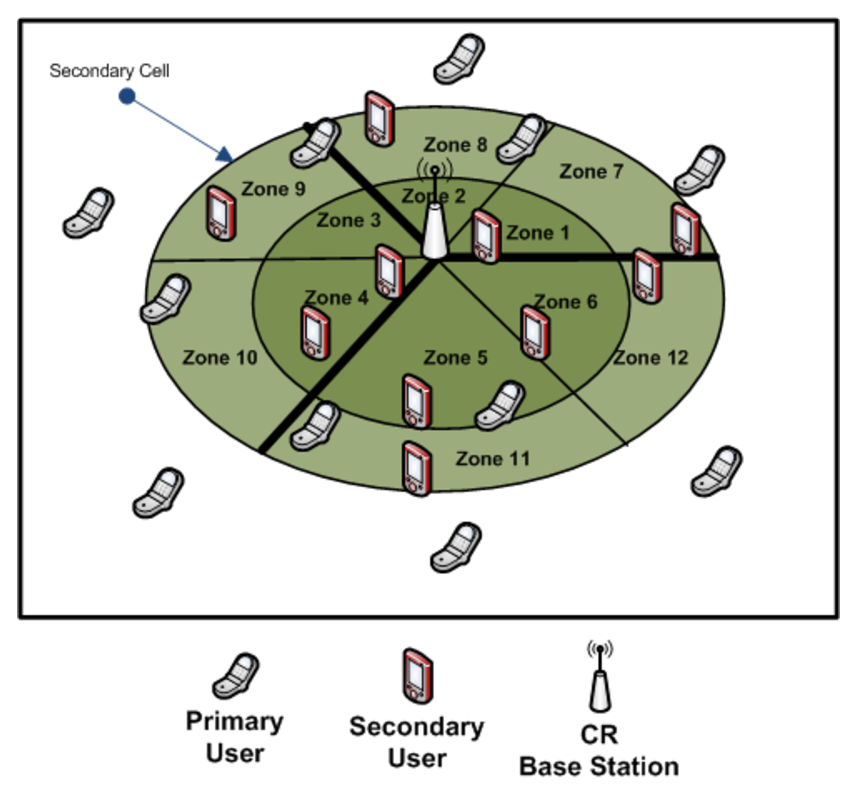
\includegraphics[width=0.99\columnwidth,keepaspectratio] {figs/cellStructure.eps}
\caption{Example zone structure.} \label{fig:zone_structure}
\end{figure}

In Figure~\ref{fig:zone_structure}, the zone structure of an infrastructure based \CR network is depicted. We assume the \CR cells are sectorized as in general practice. We further divide each sector into radial slices, and divide each slice into zones according to the distance from the base station. Each slice corresponds to an angle of $\beta$, and the radius ($r_1$, $r_2$, etc.) forms the zone structure. Thus, $(\beta, \, r_1, \, ... \, r_n)$ defines the zones in the secondary cell.

Cooperation among all SUs in the secondary cell does not improve, even worsens, the overall performance. Considering all local decisions in case of an active transmission at the edge of the cell may forbid the use of the frequency all over the cell. Similarly, considering all local decisions may result in missed detection in the close proximity of primary transmission. Therefore, we divide the cell into zones where the cooperation leads to better overall performance in terms of false alarm, missed detection, and utilization.

In each zone, all SUs broadcast their sensing measurements with low power. The first SU who broadcasts first (randomly) declares itself as the leader of the zone. The selection of the leader of the zone in this manner is achieved without any messaging overhead. Since all SUs in the zone can hear each other, the leader receives the information about spectrum sensing measurements of the other users in the zone. Therefore, the leader has the information of sensing results in the entire zone. Only the leader reports the zone's sensing decision to the \CR base station. Hence, the bandwidth requirement of the report channel is minimized.

Since the sensing results are reported for each zone separately, the \CR base station can keep track of available frequencies for each zone. A frequency can be determined as available and unavailable in different zones. So, \textbf{the Cognitive Radio system can utilize even the frequencies, which would be unavailable in other approaches, in the zones distant to the PU}.

\subsection{ZoneS sensing decision}
After sensing the signal powers locally, the SUs compare the received power with the power threshold and decide whether the channel is available or not. At that point, the decision that there is no transmission in a channel while a primary user is actually communicating is called missed detection. On the contrary, the decision that there is an ongoing transmission while no primary user is actually communicating is called false alarm. Probabilities of these occasions give the sensing reliability and sensing efficiency, respectively \cite{UpToDateSensing}. Therefore, the individual false alarm probability of a SU ($\probflocal$) becomes the probability of noise power being greater than the power threshold and the individual missed detection probability of a SU ($\probmlocal$) becomes the received power being less than the power threshold. This situation is shown in Figure \ref{fig:h0h1}.
%%%%%%%%%%%%%%%%%%%%%%%%%%%%%%%%%%%%%%%%%%%%%%%%%%%%%%%%%%%%%%%%%%%%%%%%%%%%%%%%
\begin{figure}[!htb]
\centering
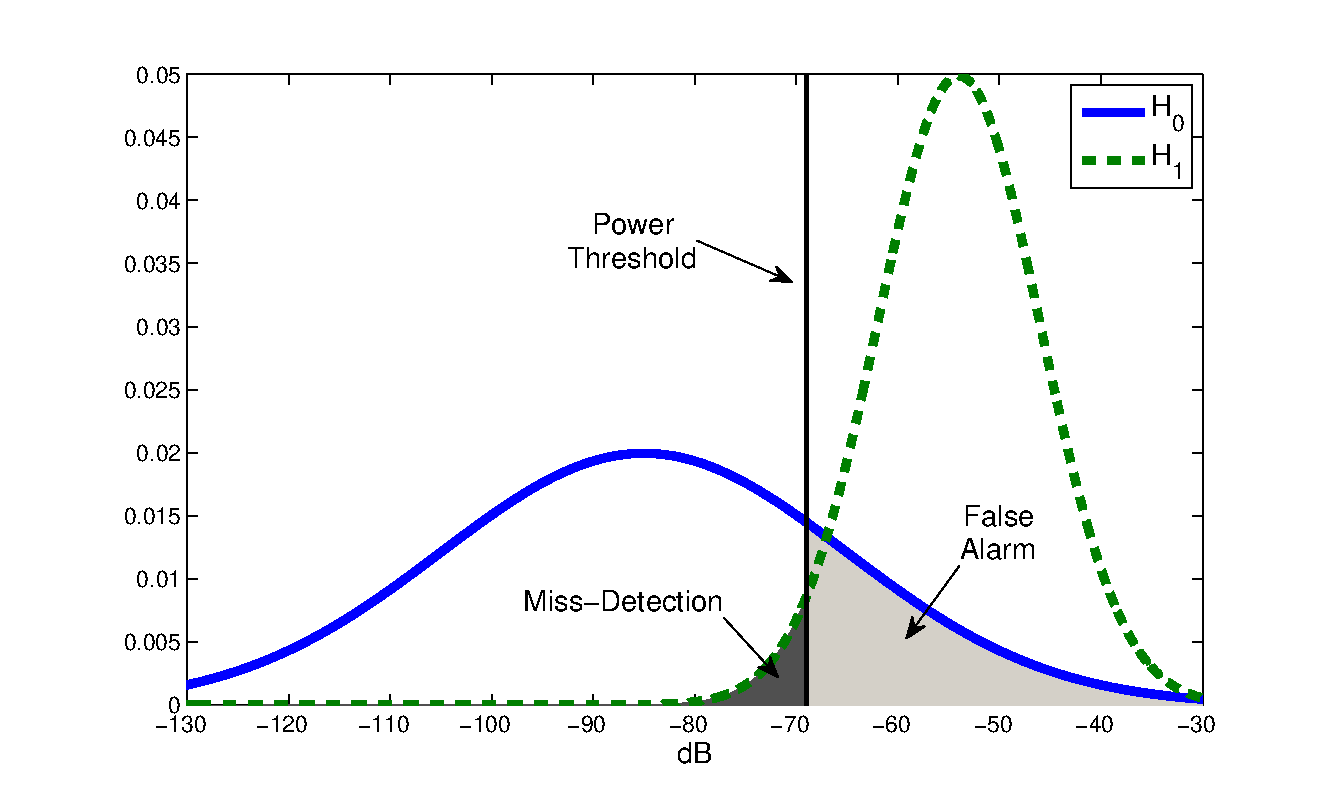
\includegraphics[width=0.99\columnwidth,keepaspectratio] {figs/h0_h1.eps}
\caption{Received Power Distributions.}
\label{fig:h0h1}
\end{figure}
%%%%%%%%%%%%%%%%%%%%%%%%%%%%%%%%%%%%%%%%%%%%%%%%%%%%%%%%%%%%%%%%%%%%%%%%%%%%%%%%

The \CR base station gathers sensing decisions zone by zone and applies the cooperation rule in each zone. Using majority as the cooperation rule yields false alarm and missed detection probabilities according to the following formulations:
%%%%%%%%%%%%%%%%%%%%%%%%%%%%%%%%%%%%%%%%%%%%%%%%%%%%%%%%%%%%%%%%%%%%%%%%%%%%%%%%
\begin{equation}
    \begin{array}{lcl}
        \probf & = & \sum\limits_{ k > \frac{N}{2}}^N {N \choose k}(\probflocal)^k\times(1-\probflocal)^{N-k} \\
        \probm & = & \sum\limits_{ k > \frac{N}{2}}^N {N \choose k}(\probmlocal)^k\times(1-\probmlocal)^{N-k}
    \end{array}
\end{equation}
%%%%%%%%%%%%%%%%%%%%%%%%%%%%%%%%%%%%%%%%%%%%%%%%%%%%%%%%%%%%%%%%%%%%%%%%%%%%%%%%

ZoneS algorithm divides the area into subareas for efficient cooperation. \textbf{These final $\probf$ and $\probm$ values are the probabilities for a single zone, not the whole cell.}

\subsection{Communication}
%%%%%%%%%%%%%%%%%%%%%%%%%%%%%%%%%%%%%%%%%%%%%%%%%%%%%%%%%%%%%%%%%%%%%%%%%%%%%%%%
\begin{figure}[!h]
\centering
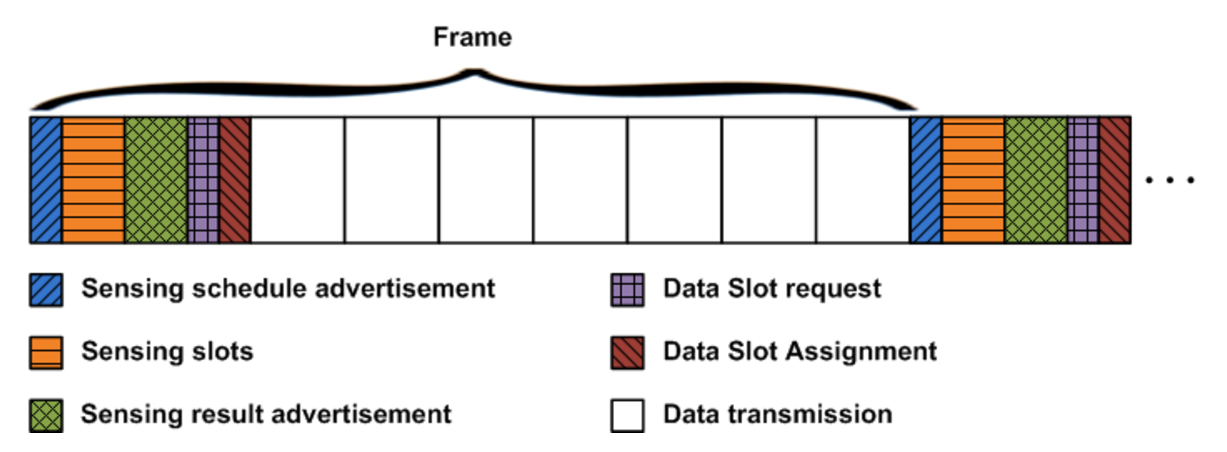
\includegraphics[width=0.99\columnwidth,keepaspectratio] {figs/frameStructure.eps}
\caption{Communication frame structure.} \label{fig:frame_structure}
\end{figure}
%%%%%%%%%%%%%%%%%%%%%%%%%%%%%%%%%%%%%%%%%%%%%%%%%%%%%%%%%%%%%%%%%%%%%%%%%%%%%%%%
In Figure~\ref{fig:frame_structure}, the communication frame structure is depicted. Each frame starts with sensing scheduling and sensing slots. A simple sensing scheduling method is assumed that assigns half of the frequencies to one half of the nodes in the zone and the other half to the remaining nodes. Collaborative sensing decision is formed and advertised after these slots. Sensing schedule advertisement, slots, and result acknowledgement are followed by communication requests and responses.

\begin{figure}[!ht]
\centering
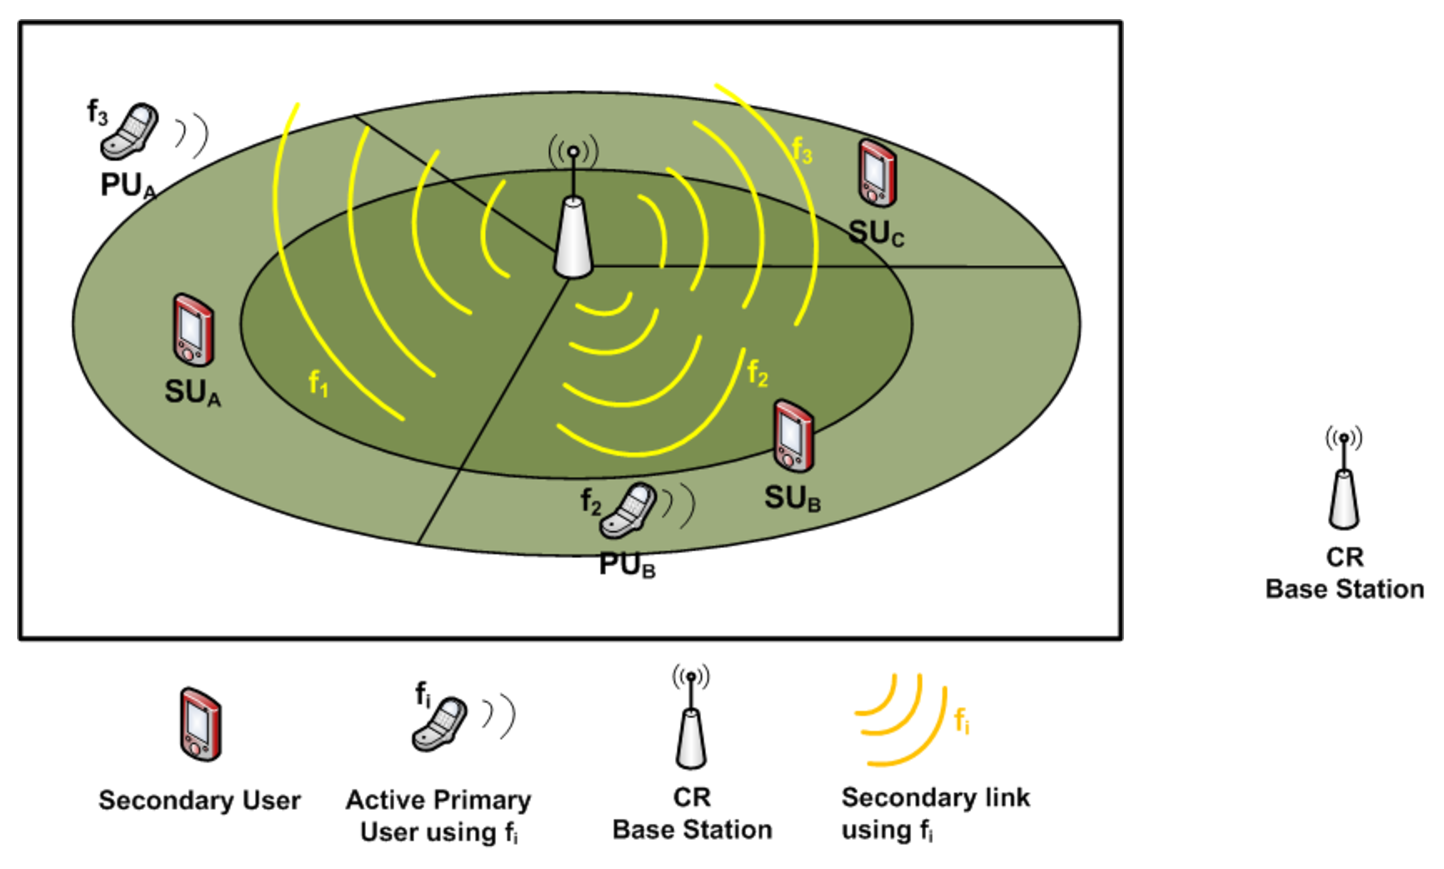
\includegraphics[width=0.99\columnwidth,keepaspectratio] {figs/communicationCases.eps}
\caption{Secondary communication.} \label{fig:network}
\end{figure}
%%%%%%%%%%%%%%%%%%%%%%%%%%%%%%%%%%%%%%%%%%%%%%%%%%%%%%%%%

After sensing part is completed, \CR base station assigns communication frequencies to the SUs who want to receive or transmit data. While choosing which frequencies to assign it takes sensing results into consideration. It can assign a frequency to a user in three cases:
\begin{enumerate}
\item No PU is actually using the channel.
\item There is a PU close by, who uses the channel, but SUs could not detect it (missed detection). This
      situation causes interference at PU and therefore collision.
\item There is a PU who uses the channel but it is not close enough to the SU, who uses the same channel,
      such that there is not a significant interference.
\end{enumerate}

These cases are illustrated in Figure \ref{fig:network}. In the figure, there is a secondary link between $SU_A$ and the CR Base over $f_1$ which is not used by any primary user. Therefore, the $SINR$ value is high enough to have a communication. There is another secondary link between $SU_C$ and the CR Base over $f_3$ which is used by $PU_A$ at other side of the cell which is far enough. Therefore, the $SINR$ value includes the interference but not so severe to degrade the communication link. Lastly, there is a secondary link between $SU_B$ and the CR Base uses $f_2$ which is also used by $PU_B$ in close proximity. In this case, collision occurs due to the miss-detection and the channel capacity decreases too much to have a valid communication. In each case the channel capacities are evaluated by the Shannon capacity formula:
%%%%%%%%%%%%%%%%%%%%%%%%%%%%%%%%%%%%%%%%%%%%%%%%%%%%%%%%%%%%%%%%%%%%%%%%%%%%%%%%
\begin{equation}
    C = B\,\, \log_2(1+SINR)
\end{equation}
%%%%%%%%%%%%%%%%%%%%%%%%%%%%%%%%%%%%%%%%%%%%%%%%%%%%%%%%%%%%%%%%%%%%%%%%%%%%%%%%
where $B$ is the bandwidth of the channel.

\section{\label{sec:results}Results}
\subsection{Simulation parameters and analysis}
Simulation parameters are shown in Table~\ref{tbl:sim_parameters}.

\begin{table}[!htb]
\renewcommand{\arraystretch}{1.2}
\caption{Simulation Parameters}
\label{tbl:sim_parameters}
\centering
\begin{tabular}{l c l}
  \hline
  Parameter & & Value\\
  \hline
  $P_{tx}$ & & -10dB \\
  $l_0$    & & 38.4dB (Urban) \\
  $\alpha$ & & 3.5 (Urban)\\
  $\mu_s$  & & 0dB\\
  $\sigma_s$ & & 8dB\\
  $\mu_0$  & & -85dB \\
  $\sigma_0$ & & 20dB \\
  $r_{cell}$ & & 1.5 km\\
  $N_{PU}$ & & 1500\\
  \hline
\end{tabular}
\end{table}
where $N_{PU}$ is the number of PUs.

As simulation output, statistics collected in terms of the false alarm, missed detection, collision, blocking of SUs, dropping of SUs, and the channel utilization by both SUs and PUs. Note that in figures we do not plot all probability values for each zone. Instead we plot their mean against number of SUs.

In simulation, radius of the \CR cell is 1.5 km, and number of PUs is 1500. Also PUs are deployed in a wider area then the SUs. They are deployed in an area with 3 km radius since we cannot assume the perfect overlapping of the primary and secondary system cells.

\subsection{$\probf$ analysis}
Figure \ref{fig:probf} illustrates the false alarm probability versus number of SUs in the cell. The probability of false alarm decreases with the increasing number of secondary users because the reliability of the cooperation decision increases with number of users cooperating. This result is expected according to the mathematical model since the cooperated false alarm probability ($\probf$) is obtained by taking powers of local false alarm probabilities ($\probflocal$).

\begin{figure}[t]
\centering
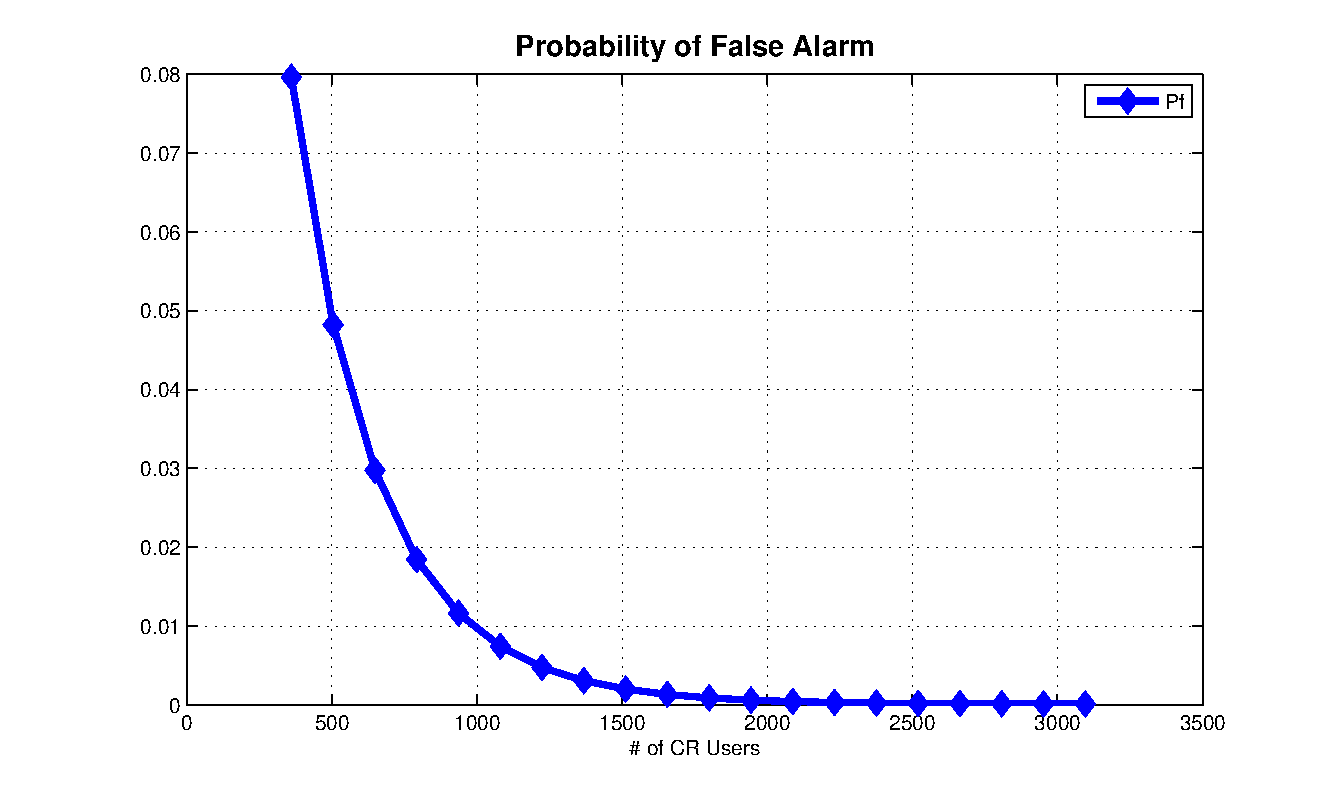
\includegraphics[width=0.99\columnwidth,keepaspectratio] {figs/pf2.eps}
\caption{Probability of False Alarm vs Number of SUs.}
\label{fig:probf}
\end{figure}

\subsection{$\probm$ and collision analysis}
Figure \ref{fig:probm} illustrates the miss-detection and collision probabilities versus the number of SUs cooperating in a zone. We observe that the probability of the miss-detection also decreases with increasing number of secondary users as in the same manner of the probability of false alarm. We also observe that collision probabilities never exceeds the missed detection probabilities. This is a reasonable result since all collisions are caused due to missed detections. Another observation from the graph is that, after some point, collision probability starts increasing. That is why, the system gets overloaded at that point.

Figure \ref{fig:probb} illustrates the blocking and dropping probabilities versus number of SUs in the cell. Both the probability of blocking and dropping stays very low for up at first but they increase almost exponentially when total utilization approaches 100 percent.

\begin{figure}[t]
\centering
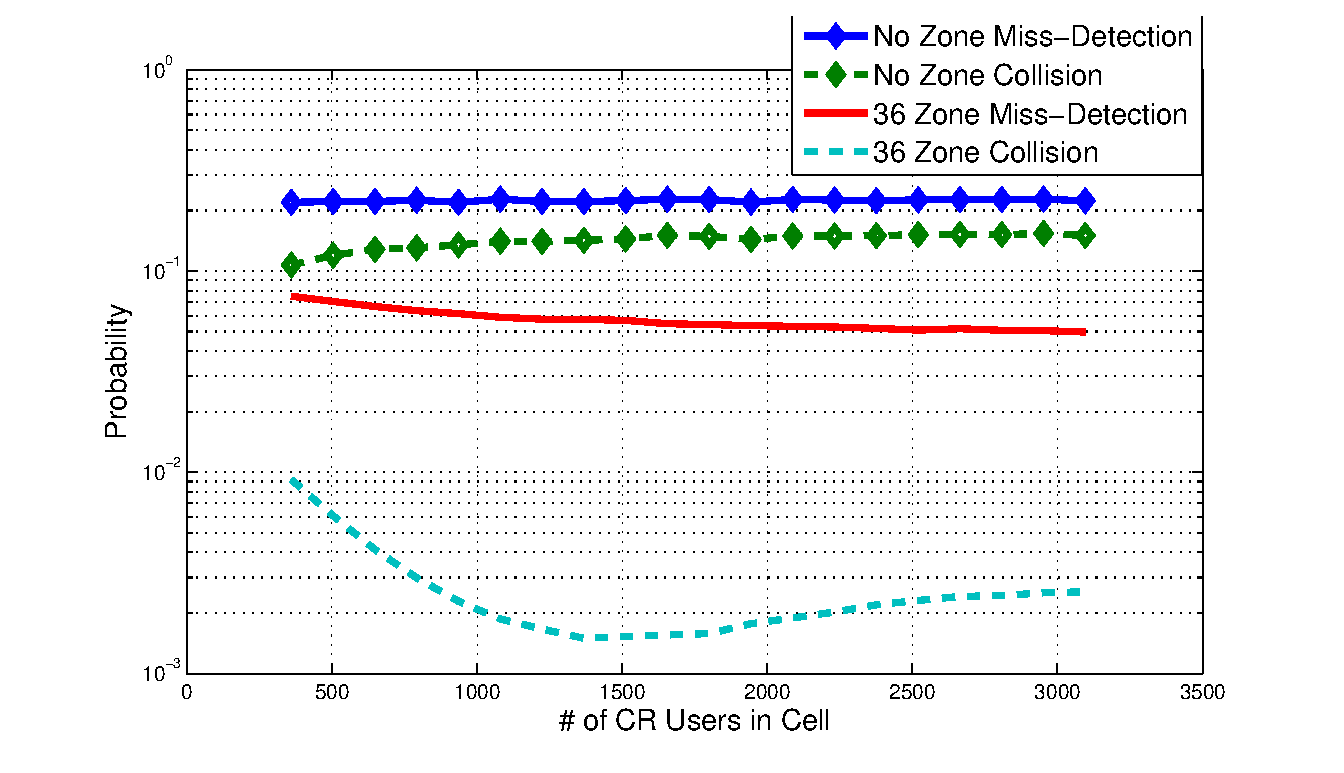
\includegraphics[width=0.99\columnwidth,keepaspectratio] {figs/pm_c.eps}
\caption{Probability of Missed Detection and Collision vs Number of
SUs} \label{fig:probm}
\end{figure}


\subsection{Utilization analysis}
Figure \ref{fig:util} illustrates the utilization of PUs, SUs, and total versus number of SUs in the cell. Since missed detection probability is not very high (almost under 4 percent all the time), utilization of primary users does not effect too much due to secondary communication. Moreover, secondary communication increases overall utilization of the wireless channels by utilizing PUs' unused spectrum. When taken into account with collision rates as increasing number of SUs, total channel utilization converges to 100 percent slower and slower.

\begin{figure}[t]
\centering
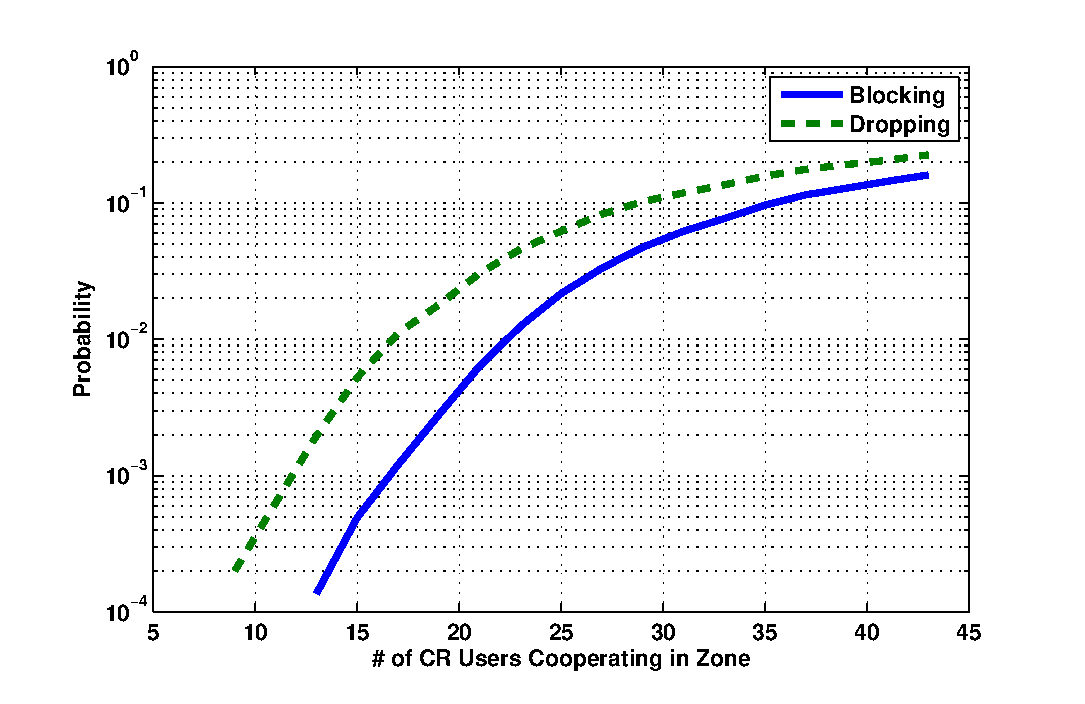
\includegraphics[width=0.99\columnwidth,keepaspectratio] {figs/pb_d.eps}
\caption{Probability of Blocking and Dropping vs Number of SUs}
\label{fig:probb}
\end{figure}

\section{\label{sec:conclusion}Conclusion}
Being aware of surroundings is the most crucial part of the \CR system since it includes sensing the environment for primary activity, finding spectrum holes and vacating the channel or adjusting the communication parameters which is a must for not to disturb the primary users.

In this paper, we focused on distributed cooperative sensing with majority cooperation rule. We observed that with a few number of SUs (~350 or less), requirements determined by standards (both probability of false alarm and missed detection should be less than 10 percent \cite{wranstandard}) cannot be satisfied. As the number of SUs increases, these requirements can be easily satisfiable but when system load becomes excessive (over 90 percent) quality of service for SUs decreases severely in terms of blocking and dropping. Moreover, due to overload in wireless channel, collision probabilities start to increase after that point.

\begin{figure}[t]
\centering
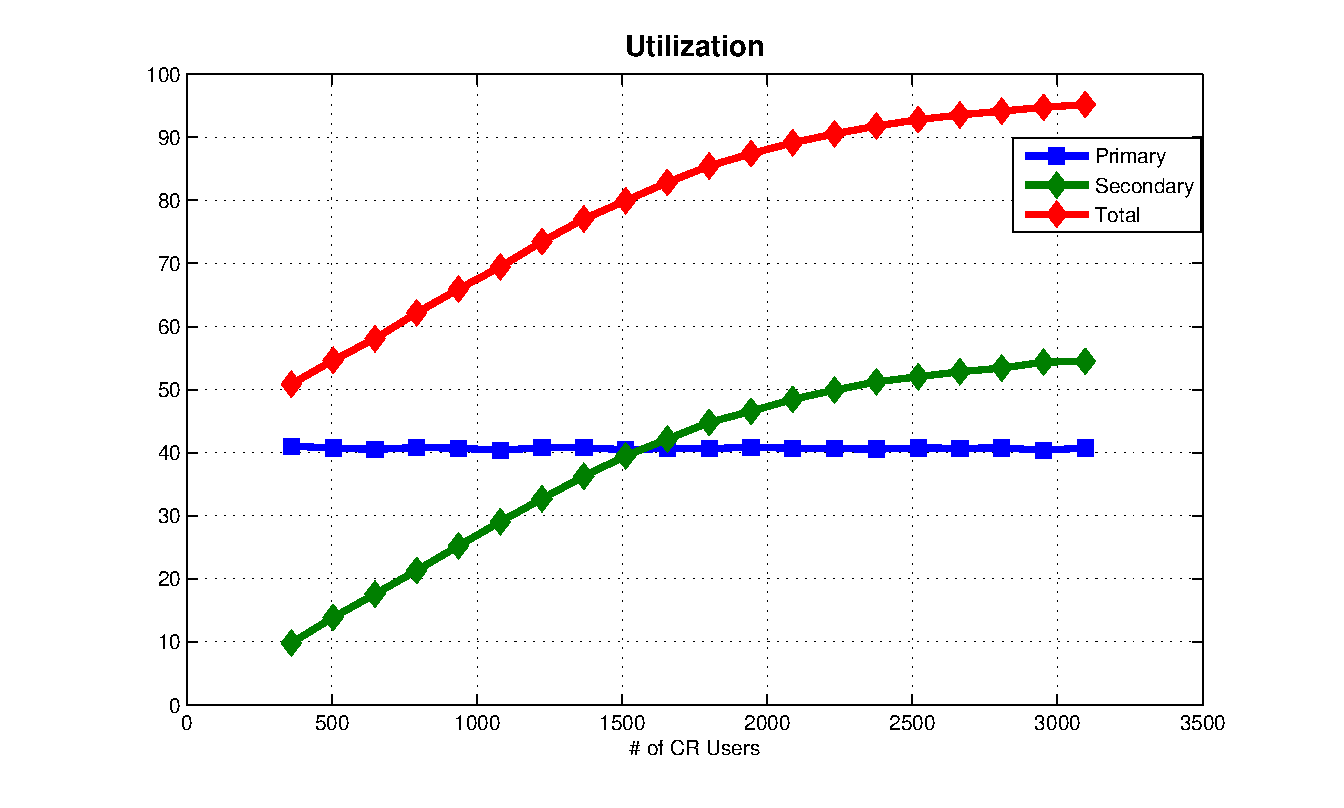
\includegraphics[width=0.99\columnwidth,keepaspectratio] {figs/utilization.eps}
\caption{Utilization of Wireless Channel} \label{fig:util}
\end{figure}

\section{\label{sec:future}Future Work}
As further improvement of this paper, we will combine our simulation with an optimization approach over sensing scheduling. Our aim at this optimization is to minimize the interference caused by secondary users by efficiently assigning the frequencies to be sensed for each secondary users.

\section*{Acknowledgment}
This work has been supported by the State Planning Organization (DPT) of Republic of Turkey under the project TAM with the Project No. 2007K120610 and COST Action IC0902 Cognitive Radio and Networking for Cooperative Coexistence of Heterogeneous Wireless Networks.

\bibliographystyle{IEEEtran}
\bibliography{bibliography}

% that's all folks
\end{document}
